\documentclass[aspectratio=169]{beamer}

\usepackage{nils-slides}
\usepackage[english]{babel}

\title[Narrative Level Detection]{Exploring Text Recombination for Automatic Narrative Level Detection}
\subtitle{LREC 2022, Marseille}
\author[]{\textbf{Nils Reiter}, Judith Sieker, Svenja Guhr, Evelyn Gius, Sina Zarrieß}
\date[]{June 2022}

\begin{document}

\maketitleframe

\begin{frame}{Narrative Level}
\begin{outline}
\1 Embedded stories, told by characters of a story
\1 Widely used phenomenon in narrative texts
\1 Crucial for content-driven narrative analysis
\1 Important for subsequent NLP tasks (e.g., coreference resolution)
\end{outline}
\pause
\begin{example}
\begin{quote}
At this the whole pack rose up into the air, and came flying down upon her: she gave a little scream, half of fright and half of anger, and tried to beat them off, \faExclamationTriangle{} and found herself lying on the bank, with her head in the lap of her sister, who was gently brushing away some dead leaves that had fluttered down from the trees upon her face.
\end{quote}
\end{example}
\end{frame}

\begin{frame}{Annotating Narrative Levels}
\begin{outline}
\1 No available corpus with annotations
\1 Shared task on guideline development \inlineslidecite{Gius2021ab}
\2 Task: Establish a guideline for annotating levels in English texts
\2 Evaluation by looking at theory, applicability (IAA), usefulness
\2 Extremely challenging annotation task, due its length
\end{outline}

\begin{block}{Contents of this Talk}
\begin{outline}
\1 Establish method to induce training data,
\1 Evaluate that it does help a model,
\1 Identify weaknesses and formulate, finally,
\1 Future paths for level detection
\end{outline}
\end{block}
\end{frame}

\begin{frame}{Outlook: Shared Task on Narrative Level Detection}
\begin{tikzpicture}[remember picture,overlay]
\node at (current page.north east) [xshift=-1cm,yshift=-1cm,anchor=north,fill=red,font=\bfseries,text=white,rotate=-45,minimum width=5cm] {In Preparation};
\end{tikzpicture}

\renewcommand\outlineii{enumerate}
\begin{outline}
\1 Shared Task with two tracks
\2 Training data generation
\3 Evaluation: Performance of a baseline BERT system
\end{outline}
\end{frame}

\begin{frame}[plain]
\begin{tikzpicture}[remember picture,overlay]
\node at (current page.center) {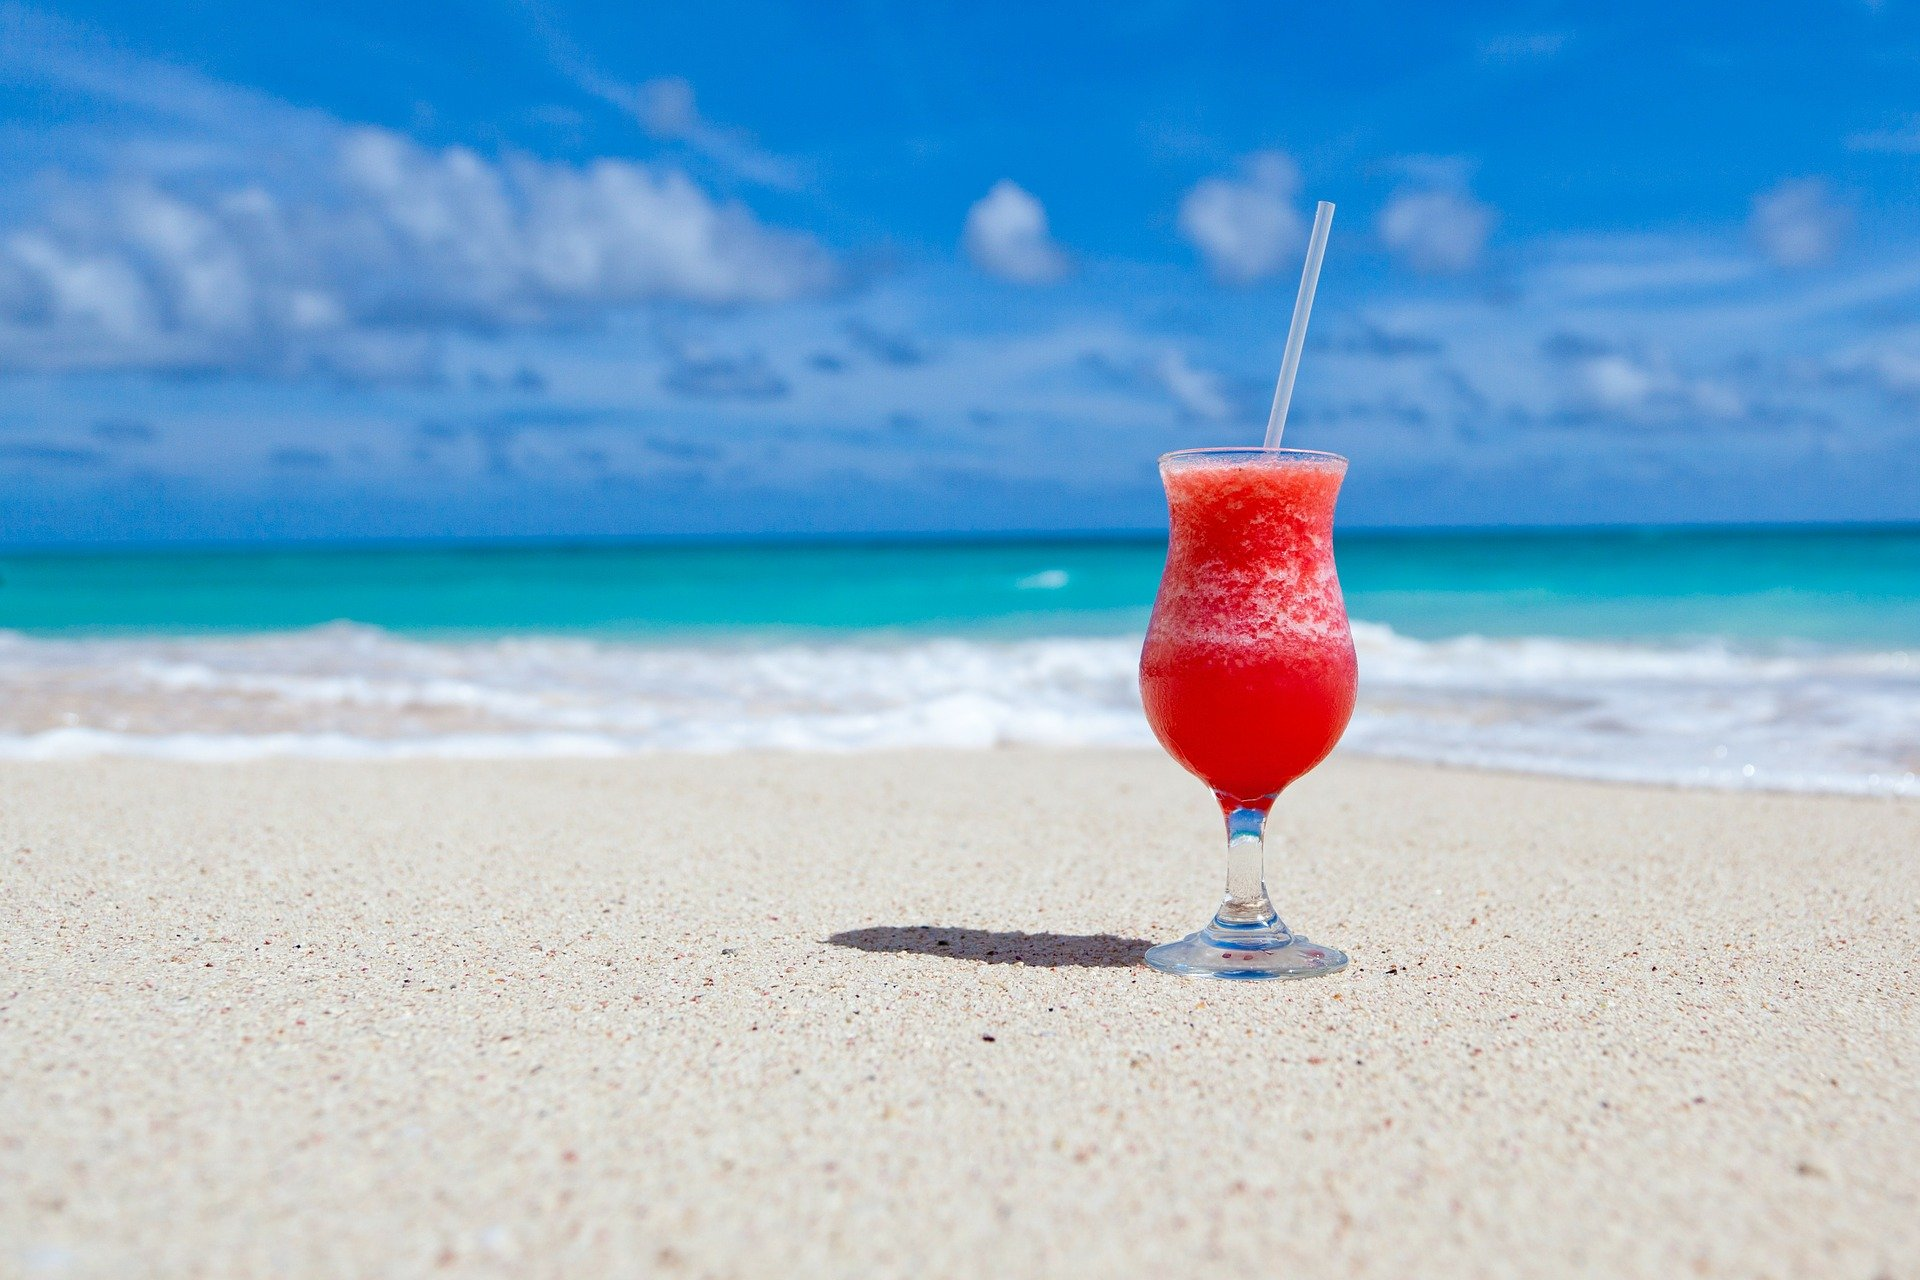
\includegraphics[width=\paperwidth]{drink-84533_1920.jpg}};
\node at (current page.center) [align=center,font=\LARGE\itshape,xshift=-3.5cm,yshift=-2.5cm] {Thank you!}; 
\end{tikzpicture}
\end{frame}

\appendix

\begin{frame}[allowframebreaks]{References}
\printbibliography
\end{frame}

\end{document}